% ******************************************************************	********************************************
%
% **************************************************************************************************************
\documentclass[ twoside,openright,titlepage,numbers=noenddot,%
								toc=bibliography,toc=listof,%
                footinclude=false,headinclude=false,cleardoublepage=empty,%
								BCOR=5mm,paper=a4,fontsize=11pt,%DIV=14,%
                ngerman%
                ]{scrreprt}

%***************************************************************************************************************
% Note: Make all your adjustments in here
%***************************************************************************************************************
% ****************************************************************************************************
% htwsaar-i-mst-config.tex 
% ****************************************************************************************************  
\RequirePackage[utf8]{inputenc}				
 \DeclareUnicodeCharacter{00A0}{~}								
\RequirePackage[T1]{fontenc} 
								
% ****************************************************************************************************
% 1. Personal data and user ad-hoc commands
% ****************************************************************************************************
\newcommand{\myTitle}{Software-Modernisierung}
\newcommand{\myDegree}{Master of Science (M.\,Sc.)\xspace}
\newcommand{\myDegreeType}{Master\xspace}
\newcommand{\myDegreeCourse}{Praktische Informatik}
\newcommand{\myName}{Nicolas Klein, Alexander Stolz\xspace}
\newcommand{\myUni}{Hochschule für Technik und Wirtschaft des Saarlandes\xspace}
\newcommand{\myCompany}{SoftwareCenter Musterhausen\xspace}
\newcommand{\myFirstProf}{Prof. Dr. Helmut Folz\xspace}
\newcommand{\myLocation}{Saarbrücken\xspace}
\newcommand{\myTime}{27.~Juli~2021\xspace}
\newcommand{\currentVersion}{Version 2.1\xspace} % TODO: ggf. über git Versionsinformationen automatisch bereitstellen und verwenden

% ********************************************************************
% Setup, finetuning, and useful commands
% ********************************************************************
\newcounter{dummy} % necessary for correct hyperlinks (to index, bib, etc.)
% ****************************************************************************************************


% ****************************************************************************************************
% 2. Loading some handy packages
% ****************************************************************************************************
% ******************************************************************** 
% Packages with options that might require adjustments
% ******************************************************************** 
\PassOptionsToPackage{ngerman}{babel}   % change this to your language(s)
 \RequirePackage{babel}					
 \RequirePackage{csquotes}
	
\PassOptionsToPackage{language=auto,style=numeric-comp,backend=bibtex8,bibencoding=ascii,maxbibnames=50}{biblatex}
 \RequirePackage{biblatex}	
 \bibliography{Bibliography}			

\PassOptionsToPackage{fleqn}{amsmath}		% math environments and more by the AMS 
 \RequirePackage{amsmath}

% ******************************************************************** 
% Setting up the page and margins
% ******************************************************************** 
\usepackage{geometry}
 \geometry{a4paper,left=25mm,right=35mm,top=25mm,bottom=30mm}
% DIESE WERTE SIND NICHT ZU VERÄNDERN -- DO NOT CHANGE THESE VALUES

% ******************************************************************** 
% General useful packages
% ******************************************************************** 
%\usepackage[automark]{scrpage2}
\PassOptionsToPackage{dvipsnames}{xcolor}
	\RequirePackage{xcolor} % [dvipsnames]  
	\definecolor{ingwi}{cmyk}{.9,0,0,0}
\usepackage{textcomp} % fix warning with missing font shapes
\usepackage{scrhack} % fix warnings when using KOMA with listings package          
\usepackage{xspace} % to get the spacing after macros right  
\usepackage{mparhack} % get marginpar right
%\usepackage{fixltx2e} % fixes some LaTeX stuff <-- ist seit 2015 nicht mehr notwendig
\PassOptionsToPackage{printonlyused}{acronym}
	\usepackage{acronym} % nice macros for handling all acronyms in the thesis
%\renewcommand{\bflabel}[1]{{#1}\hfill} % fix the list of acronyms
\usepackage{booktabs}
\usepackage{multirow}
\usepackage[shadow]{todonotes} %Settings for ToDoNotes
% Eigene Shortcuts fuer laengere Befehle
	\newcommand{\todox}[1]{\todo[inline, size=\small]{#1}}
	%Nummerierte Anmerkungen
	\newcounter{todocounter}
	\renewcommand{\todox}[2][]{\stepcounter{todocounter}\todo[inline, size=\small,caption={\thetodocounter: #2}, #1]{\renewcommand{\baselinestretch}{0.5}\selectfont\thetodocounter: #2\par}}
\usepackage{blindtext}
%\usepackage{footmisc}

% ****************************************************************************************************


% ****************************************************************************************************
% 3. Setup floats: tables, (sub)figures, and captions
% ****************************************************************************************************
\usepackage{tabularx} % better tables
	\setlength{\extrarowheight}{3pt} % increase table row height
%\newcommand{\myfloatalign}{\centering} % to be used with each float for alignment
\usepackage{caption}
\captionsetup{format=hang,font=small}
\usepackage{subfig}
\usepackage{wrapfig}
\usepackage{nameref}
% ****************************************************************************************************


% ****************************************************************************************************
% 6. Setup code listings
% ****************************************************************************************************
\usepackage{listings} 
%\lstset{emph={trueIndex,root},emphstyle=\color{BlueViolet}}%\underbar} % for special keywords
\lstset{language=[LaTeX]Tex,%C++,
    keywordstyle=\color{RoyalBlue},%\bfseries,
    basicstyle=\small\ttfamily,
    %identifierstyle=\color{NavyBlue},
    commentstyle=\color{Green}\ttfamily,
    stringstyle=\rmfamily,
    numbers=none,%left,%
    numberstyle=\scriptsize,%\tiny
    stepnumber=5,
    numbersep=8pt,
    showstringspaces=false,
    breaklines=true,
    frameround=ftff,
    frame=single,
		texcl=true,
    belowcaptionskip=.75\baselineskip
    %frame=L
} 
%Styles für verschiedene Sprachen festlegen, z.B. Java
\lstdefinestyle{Java}{
belowcaptionskip=1\baselineskip,
  breaklines=true,
  xleftmargin=\parindent,
  language=Java,
	texcl=true,
  showstringspaces=false,
  basicstyle=\footnotesize\ttfamily,
  keywordstyle=\bfseries\color{green!40!black},
  commentstyle=\itshape\color{purple!40!black},
  identifierstyle=\color{blue},
  stringstyle=\color{orange}}
% ****************************************************************************************************    		   


% ****************************************************************************************************
% 6. PDFLaTeX, hyperreferences and citation backreferences
% ****************************************************************************************************
% ********************************************************************
% Using PDFLaTeX
% ********************************************************************
\PassOptionsToPackage{pdftex,hyperfootnotes=false,pdfpagelabels}{hyperref}
	\usepackage{hyperref}  % backref linktocpage pagebackref
\pdfcompresslevel=9
\pdfadjustspacing=1 
\PassOptionsToPackage{pdftex}{graphicx}
	\usepackage{graphicx} 
    

% ********************************************************************
% Hyperreferences
% ********************************************************************
\hypersetup{%
    %draft,	% = no hyperlinking at all (useful in b/w printouts)
    pdfstartpage=1, pdfstartview=Fit,%
		colorlinks=true, linktocpage=true,
		%urlcolor=Black, linkcolor=Black, citecolor=Black, %pagecolor=Black,%
		%urlcolor=brown, linkcolor=RoyalBlue, citecolor=green, %pagecolor=RoyalBlue,%
    % uncomment the following line if you want to have black links (e.g., for printing)
    colorlinks=false, pdfborder={0 0 0},
    breaklinks=true, pdfpagemode=UseNone, pageanchor=true, pdfpagemode=UseOutlines,%
    plainpages=false, bookmarksnumbered, bookmarksopen=true, bookmarksopenlevel=1,%
    hypertexnames=true, pdfhighlight=/O,%nesting=true,%frenchlinks,%
    pdftitle={\myTitle},%
    pdfauthor={\textcopyright\ \myName, \myUni},%
    pdfsubject={},%
    pdfkeywords={},%
    pdfcreator={pdfLaTeX},%
    pdfproducer={LaTeX with hyperref}%
}   

% ********************************************************************
% Setup autoreferences
% ********************************************************************
% There are some issues regarding autorefnames
% http://www.ureader.de/msg/136221647.aspx
% http://www.tex.ac.uk/cgi-bin/texfaq2html?label=latexwords
% you have to redefine the makros for the 
% language you use, e.g., american, ngerman
% (as chosen when loading babel/AtBeginDocument)
% ********************************************************************
\makeatletter
\@ifpackageloaded{babel}%
    {%
       \addto\extrasamerican{%
					\renewcommand*{\figureautorefname}{Figure}%
					\renewcommand*{\tableautorefname}{Table}%
					\renewcommand*{\partautorefname}{Part}%
					\renewcommand*{\chapterautorefname}{Chapter}%
					\renewcommand*{\sectionautorefname}{Section}%
					\renewcommand*{\subsectionautorefname}{Section}%
					\renewcommand*{\subsubsectionautorefname}{Section}% 	
				}%
       \addto\extrasngerman{% 
					\renewcommand*{\chapterautorefname}{Kapitel}%
					\renewcommand*{\sectionautorefname}{Abschnitt}%
					\renewcommand*{\subsectionautorefname}{Abschnitt}%
					\renewcommand*{\subsubsectionautorefname}{Abschnitt}% 
					\renewcommand*{\paragraphautorefname}{Absatz}%
					\renewcommand*{\subparagraphautorefname}{Absatz}%
					\renewcommand*{\footnoteautorefname}{Fu\"snote}%
					\renewcommand*{\FancyVerbLineautorefname}{Zeile}%
					\renewcommand*{\theoremautorefname}{Theorem}%
					\renewcommand*{\appendixautorefname}{Anhang}%
					\renewcommand*{\equationautorefname}{Gleichung}%        
					\renewcommand*{\itemautorefname}{Punkt}%
				}%	
			% Fix to getting autorefs for subfigures right (thanks to Belinda Vogt for changing the definition)
			\providecommand{\subfigureautorefname}{\figureautorefname}%  			
    }{\relax}
\makeatother


% ****************************************************************************************************
% 6. Last calls before the bar closes
% ****************************************************************************************************
% ********************************************************************
% Development Stuff
% ********************************************************************
%\listfiles
\PassOptionsToPackage{l2tabu,orthodox,abort}{nag}
	\usepackage{nag}
%\PassOptionsToPackage{warning, all}{onlyamsmath}
%	\usepackage{onlyamsmath}


% ****************************************************************************************************
% 7. Further adjustments (experimental)
% ****************************************************************************************************
%\usepackage{tocbibind} %Allows us to add Bibliography to ToC
\usepackage{enumitem}
\setdescription{font=\normalfont\bfseries} %Changes the appearance of description items
\usepackage[activate={true,nocompatibility},final,tracking=true,kerning=true,spacing=true,factor=1100,stretch=10,shrink=10]{microtype}


% ********************************************************************
% Using different fonts
% ********************************************************************
%\usepackage{lmodern} % <-- no osf support :-(
%\usepackage[tt=false]{libertine} % [osf]
%\usepackage{luximono} 
\usepackage{mathpazo} 
%\usepackage[urw-garamond]{mathdesign} <-- no osf support :-(

\setkomafont{disposition}{\bfseries}
% ****************************************************************************************************

%********************************************************************
% Hyphenation
%*******************************************************
%\hyphenation{put special hyphenation here}

% ********************************************************************
% GO!GO!GO! MOVE IT!
%*******************************************************
\begin{document}
\frenchspacing
\raggedbottom
\selectlanguage{ngerman} % american ngerman
\pagenumbering{roman}
\pagestyle{plain}
%*******************************************************
% Frontmatter
%*******************************************************
%*******************************************************
% Titlepage
%*******************************************************
\begin{titlepage}\linespread{1.5}\selectfont

\includegraphics[width=\linewidth]{Graphics/htwsaar_Logo_inwi_head_VF_4C_crop}
  \begin{center}
    \large  
    \hfill
    \vfill
		
		\bigskip
		Ausarbeitung für das Pflichtmodul
    Software-Entwicklungsprozesse \\
    
    an der \myUni \\
    im Studiengang \myDegreeCourse \\
    der Fakultät für Ingenieurwissenschaften \\ 
    
  \vfill
	
  \begingroup
    \Large\bfseries\myTitle 
  \endgroup
	
	\bigskip
	
   von \\
  \myName
	
  \vfill
	
  begutachtet von \\
  \myFirstProf \\

  \vfill
	
  \myLocation, \myTime                   

    \end{center}       
\end{titlepage}   
\cleardoublepage%*******************************************************
% Declaration
%*******************************************************
\pdfbookmark[0]{Selbständigkeitserklärung}{declaration}
\chapter*{Selbständigkeitserklärung}
%\thispagestyle{empty}

Ich versichere, dass ich die vorliegende Arbeit (bei einer Gruppenarbeit: den entsprechend gekennzeichneten
Anteil der Arbeit) selbständig verfasst und keine anderen als die angegebenen Quellen und
Hilfsmittel benutzt habe.

Ich erkläre hiermit weiterhin, dass die vorgelegte Arbeit zuvor weder von mir noch von einer anderen Person an dieser oder einer
anderen Hochschule eingereicht wurde.

Darüber hinaus ist mir bekannt, dass die Unrichtigkeit dieser Erklärung eine Benotung der 
Arbeit mit der Note \glqq nicht ausreichend\grqq zur Folge hat und einen Ausschluss von der Erbringung 
weiterer Prüfungsleistungen zur Folge haben kann.
\bigskip
 
\noindent\textit{\myLocation, \myTime}

\smallskip

\begin{flushright}
    \begin{tabular}{m{5cm}}
        \\ \hline
        \centering\myName \\
    \end{tabular}
\end{flushright}
%\cleardoublepage%*******************************************************
% Sperrvermerk
%*******************************************************
% Der Sperrvermerk kann entfernt werden, wenn die Arbeit z.B. nicht im 
% Zusammenarbeit mit einem Unternehmen angefertigt wurde oder kein
% Sperrvermerk verlangt wird.

\pdfbookmark[0]{Sperrvermerk}{sperrvermerk}
\chapter*{Sperrvermerk}
%\thispagestyle{empty}

Die vorliegende Arbeit mit dem Titel "`\myTitle"' enthält vertrauliche Daten des Unternehmens \myCompany.

Die Arbeit darf nur dem Erst- und Zweitgutachter sowie befugten Mitgliedern des Prüfungsausschusses zugänglich gemacht werden. 
Eine Veröffentlichung und Vervielfältigung der Arbeit ist -- auch in Auszügen -- nicht gestattet.

Eine Einsichtnahme der Arbeit durch Unbefugte bedarf einer ausdrücklichen Genehmigung des Verfassers und des Unternehmens \myCompany.
 % <-- sollte in der Regel nicht notwendig sein und mit Betreuer/Unternehmen abgeklärt werden
%\cleardoublepage%*******************************************************
% Abstract
%*******************************************************
\pdfbookmark[0]{Zusammenfassung}{Zusammenfassung}
\chapter*{Zusammenfassung}
Kurze Zusammenfassung des Inhaltes in deutscher Sprache, der Umfang beträgt zwischen einer halben und einer ganzen DIN A4-Seite.

Orientieren Sie sich bei der Aufteilung bzw. dem Inhalt Ihrer Zusammenfassung an Kent Becks Artikel: \url{http://plg.uwaterloo.ca/~migod/research/beckOOPSLA.html}. % <-- Auskommentiert
\cleardoublepage%*******************************************************
% Acknowledgments
%*******************************************************
\pdfbookmark[0]{Danksagung}{acknowledgments}

% Beispiel für ein sinnvolles Zitat 


\bigskip



\cleardoublepage%*******************************************************
% Table of Contents
%*******************************************************
\setcounter{tocdepth}{2} % <-- 2 includes up to subsections in the ToC
\setcounter{secnumdepth}{3} % <-- 3 numbers up to subsubsections

\pdfbookmark[0]{\contentsname}{toc}
\tableofcontents 

% Die weiteren Verzeichnisse folgen am Ende des Dokuments 

                  


%*******************************************************
% Mainmatter
%*******************************************************
\cleardoublepage
\pagenumbering{arabic}
\pagestyle{headings}
%\pagestyle{scrheadings}
%\cleardoublepage\chapter{Einleitung}
Sofern eine Software in Benutzung ist, muss sie angepasst und verbessert werden. \cite{lehman_understanding_1979}\\
Dies zeigte sich bei der Einführung der \acs{DSGVO} \cite{noauthor_datenschutz-grundverordnung_nodate}. Letztere stellte unter anderem neue Anforderung an den Umgang mit personenbezogenen Daten. Bestehende Software-Systeme müssen sich diesen Anforderungen stellen. Wegen nicht-Beachtung dieser Anforderungen musste der Bekleidungshersteller H\&M im Jahr 2020 ein Bußgeld von 35,3 Millionen Euro zahlen \cite{the_hamburg_commissioner_for_data_protection_and_freedom_of_information_353_2020}.\\
Um auf äußere Einflüsse zu reagieren, muss eine Software folglich stets flexibel bleiben. Eine flexible Software kann auch an neue Anforderungen angepasst werden. Allerdings widerstehen, über viele Jahre gewachsene Software-Systeme, meist Änderungen.\\\\
Die Einführung der DSGVO zeigt anschaulich, dass diese Flexibilität einer Software essenziell für den Betrieb und Verkauf dieser ist. Neue Anforderungen können durch den Gesetzgeber formuliert werden. Anschließend muss diesen Folge geleistet werden.\\
Neben dem Gesetzgeber muss die Software auch flexibel auf die Konkurrenz reagieren können. Neue Vertriebskonzepte wie Software as a Service (SaaS) halten zunehmend mehr Einzug in der IT-Branche. Um diesen Markt bedienen zu können, muss die Software ebenfalls angepasst werden.\\
Die Frage nach der Flexibilität einer Software ist folglich nicht nebensächlich. Eine unflexible Software wird zunehmend weniger wettbewerbsfähig. Um am Markt relevant zu bleiben, muss die Flexibilität einer Software erhalten bleiben.\\\\
In dieser Arbeit werden die Gründe für eine Software-Modernisierung aufgearbeitet und konkrete Maßnahmen für eine Modernisierung der Software betrachten. 

\section{Struktur der Arbeit}
Die Arbeit ist dabei wie folgt strukturiert. Zunächst wird in Kapitel \ref{chapter2} analysiert, warum eine Software-Modernisierung benötigt wird. Kapitel \ref{chapter3} ordnet die Software-Modernisierung in den Software-Entwicklungszyklus ein. In Kapitel \ref{chapter4} wird auf das Refactoring und dessen Bedeutung für die Software-Modernisierung eingegangen. Kapitel \ref{ch:vorgehensmodell} wird das Cloud-Computing betrachten und dessen Bedeutung für die Software-Modernisierung aufzeigen. Im letzten Kapitel wird abschließend ein konkretes Vorgehensmodell für eine Modernisierung mittels des Cloud-Computings vorgestellt.	 	% Diese Einbindungen werden natürlich entfernt, wenn es an die richtige
% <<< Hier alle Chapter der Abschlussarbeit (einzeln) einbinden

%Einleitung
\cleardoublepage\chapter{Einleitung}
Sofern eine Software in Benutzung ist, muss sie angepasst und verbessert werden. \cite{lehman_understanding_1979}\\
Dies zeigte sich bei der Einführung der \acs{DSGVO} \cite{noauthor_datenschutz-grundverordnung_nodate}. Letztere stellte unter anderem neue Anforderung an den Umgang mit personenbezogenen Daten. Bestehende Software-Systeme müssen sich diesen Anforderungen stellen. Wegen nicht-Beachtung dieser Anforderungen musste der Bekleidungshersteller H\&M im Jahr 2020 ein Bußgeld von 35,3 Millionen Euro zahlen \cite{the_hamburg_commissioner_for_data_protection_and_freedom_of_information_353_2020}.\\
Um auf äußere Einflüsse zu reagieren, muss eine Software folglich stets flexibel bleiben. Eine flexible Software kann auch an neue Anforderungen angepasst werden. Allerdings widerstehen, über viele Jahre gewachsene Software-Systeme, meist Änderungen.\\\\
Die Einführung der DSGVO zeigt anschaulich, dass diese Flexibilität einer Software essenziell für den Betrieb und Verkauf dieser ist. Neue Anforderungen können durch den Gesetzgeber formuliert werden. Anschließend muss diesen Folge geleistet werden.\\
Neben dem Gesetzgeber muss die Software auch flexibel auf die Konkurrenz reagieren können. Neue Vertriebskonzepte wie Software as a Service (SaaS) halten zunehmend mehr Einzug in der IT-Branche. Um diesen Markt bedienen zu können, muss die Software ebenfalls angepasst werden.\\
Die Frage nach der Flexibilität einer Software ist folglich nicht nebensächlich. Eine unflexible Software wird zunehmend weniger wettbewerbsfähig. Um am Markt relevant zu bleiben, muss die Flexibilität einer Software erhalten bleiben.\\\\
In dieser Arbeit werden die Gründe für eine Software-Modernisierung aufgearbeitet und konkrete Maßnahmen für eine Modernisierung der Software betrachten. 

\section{Struktur der Arbeit}
Die Arbeit ist dabei wie folgt strukturiert. Zunächst wird in Kapitel \ref{chapter2} analysiert, warum eine Software-Modernisierung benötigt wird. Kapitel \ref{chapter3} ordnet die Software-Modernisierung in den Software-Entwicklungszyklus ein. In Kapitel \ref{chapter4} wird auf das Refactoring und dessen Bedeutung für die Software-Modernisierung eingegangen. Kapitel \ref{ch:vorgehensmodell} wird das Cloud-Computing betrachten und dessen Bedeutung für die Software-Modernisierung aufzeigen. Im letzten Kapitel wird abschließend ein konkretes Vorgehensmodell für eine Modernisierung mittels des Cloud-Computings vorgestellt.

%Lehmanns Gesetze
\cleardoublepage\chapter{Lehmanns-Gesetze}
\label{chapter2}
In diesem Kapitel wird auf Lehmanns Gesetze eingegangen. Hierbei werden zunächst die Personen Lehmann und Bélády betrachtet.\\
Anschließend werden das erste und zweite der Gesetze von Lehmann und Bélády erläutert. Mit diesem Wissen können einige inneren und äußeren Ursachen für Lehmanns Gesetze analysiert werden.\\
Das Kapitel schließt mit den langfristigen Auswirkungen von Lehmanns Gesetzen. 

\section{Die Personen Lehmann und Bélády}
Die Zusammenhänge zwischen Benutzung und Anpassung der Software wurden schon früh in der Informatik erkannt. Der Informatik-Professor Manny Lehman und der Informatiker László Bélády formulierten zwischen 1974 und 1996 eine Reihe von Gesetzen. Diese nannten sie die “Laws of Software-Evolution“. Die Gesetze beschreiben ein Gleichgewicht zwischen Kräften, die neue Entwicklungen vorantreiben, auf der einen Seite und Kräften, die den Fortschritt bremsen, auf der anderen Seite. \cite{lehman_understanding_1979}

\subsection{Korrektheit von Lehmanns Gesetzen}
Lehmanns und Bélády’s Gesetze sind weniger Gesetze, als es Beobachtungen sind. Die Korrektheit dieser Beobachtungen wurde bereits in vielen Systemen und Anwendungen untersucht und validiert.\\
Ein Beispiel dafür wäre die Arbeit von Feitelson et al. \cite{israeli_linux_2010}. In dieser wurden 810 Version des Linux-Kernels, welche über ein Zeitraum von 14 Jahren veröffentlicht wurden, nach der Evolution des Software-Systems charakterisiert. Als Basis wurden Lehmanns Gesetze angenommen und diese mit verschiedensten Metriken nachgewiesen. \\
Zum Beispiel wurde das System-Wachstum anhand von Codezeilen oder der Anzahl von Funktionen quantifiziert. Darüber hinaus wurde das funktionale Wachstum von Linux anhand der Anzahl von Systemaufrufen gemessen.\\
Dabei konnten das erste und zweite von Lehmanns Gesetzen nachgewiesen werden. Auf diese wird im Folgenden eingegangen.

\subsection{Das erste und zweite Gesetz}
Lehmann und Bélády haben im ersten Gesetz schon 1974 erkannt, dass eine Änderung und Umstrukturierung eines Software-Systems stattfindet. Vorausgesetzt das Software-System wird aktiv genutzt. Ferner wurde im zweiten Gesetz erkannt, dass der Effekt dieser Änderung negativ ist. Außer es wird ein zusätzlicher Aufwand unternommen, um dem entgegenzuwirken.
\pagebreak

\section{Gründe für Lehmanns Gesetze}
Nachdem Feitelson et al. die Gültigkeit von Lehmanns Gesetzen festgestellt hat, gilt es zu fragen, warum diese Gesetze gelten. Ausgangspunkt dafür sind äußere und innere Kräfte, welche auf die Software einwirken.\\
Auf diese beiden Kräfte wird im Folgenden eingegangen.

\subsection{Äußere Gründe für Lehmanns Gesetze}
Ein Softwaresystem ist nicht isoliert zu betrachten. Es ist in eine Umgebung eingebettet. Grundsätzlich besteht ein Bedarf an Anpassungen, wenn sich die Umgebung der Software wandelt.\cite{bommer_softwarewartung_2016} Hierfür werden im Folgenden einige mögliche Gründe aufgeführt:

\begin{itemize}
    \item Beispiel für die fachliche Umgebung einer Software wären neue Compliance-Anforderungen. Wird eine Software über viele Jahre oder Jahrzehnte genutzt, sind Gesetzesänderungen zu erwarten. Folglich muss eine, sich in der Benutzung befindende, Software darauf reagieren.
    \item Auch ein Umdenken in der Geschäftsstrategie ist ein möglicher äußerer Faktor. Neue Märkte haben neue Anforderungen. Ein Beispiel hierfür wäre das Expandieren nach China. Im fern-östlichen Raum gelten nicht nur andere Gesetze, sondern auch andere Sitten. Dies kann umfangreiche Änderungen an der Software nach sich ziehen.
    \item Darüber hinaus kann auch ein neues Vertriebsmodell für Veränderung sorgen. Beispiele hierfür wären Geschäftsmodelle wie \ac{SaaS}. Auf \acs{SaaS} wird im Rahmen des letzten Kapitels umfangreicher eingegangen.
    \item Abschließend kann auch ein Fortschritt der Technik Auslöser für eine Reihe von neuen Anforderungen sein. Neue Programmiersprachen und Frameworks können ein schnelleres Voranschreiten in der Entwicklung ermöglichen. Letzteres wiederum kann so die Zeit zwischen der Entwicklung und dem ersten Release verkürzen. Auch Fehler im System können möglicherweise schneller behoben werden. Sollte die Konkurrenz die genannten Vorteile erzielen, kann dies ein Wettbewerbsvorteil für die Konkurrenz sein.
\end{itemize}

\subsection{Innere Gründe für Lehmanns Gesetze}
Neben den bereits beschriebenen äußeren Einflüssen führen auch eine Reihe von inneren Gründen zu Lehmanns Gesetzen. Die Software erfährt auch ein Wandel der technischen Umgebung. Im Folgenden werden hierfür einige Beispiele angeführt:

\begin{itemize}
    \item Seacord et al. \cite{seacord_modernizing_2003} führt als ersten Grund Verbesserungen an dem Produkt selbst an. Hierzu gehört Fehlerverbesserungen und Performance-Optimierungen. Neue Komponenten werden hinzugefügt, existierende Komponenten angepasst. \cite{seacord_modernizing_2003}
    \item Während der Definitions-Phase der Architektur kann ein Grad von Anpassungsfähigkeit und Flexibilität eingeplant werden. Jedoch sind nicht die Anforderungen bekannt, welche erst in der Zukunft gestellt werden. Die Architektur kann nicht für diese ausgelegt werden. Folglich degeneriert die Architektur zunehmend.\cite{seacord_modernizing_2003}\cite{daniel_kramer_legacy-software_2020}
    \item Darüber hinaus wächst die Code-Basis. Wiederholte Modifikation führt meist zu mehr Code und komplexerer Software. Das System wird folglich brüchiger. Die Wahrscheinlichkeit von Seiteneffekten nimmt zu, mit jeder Änderung die eingearbeitet wird. Die Wartung der Software wird folglich Schritt für Schritt schwieriger. Letzteres verlangt nach mehr Personal und nach speziell geschulten Personal. \cite{seacord_modernizing_2003}\cite{daniel_kramer_legacy-software_2020}
    \item Abschließend ist es möglich, dass neue Mitarbeiter an der Software arbeiten. Die ursprünglichen Mitarbeiter, welche die Architektur der Software entwickelt haben, sind möglicherweise nicht mehr in der Firma beschäftigt oder im Ruhestand. Spätestens jetzt können Verständnisprobleme mit der Definition der Architektur oder der bestehenden Code-Basis aufkommen.\\
    Fehlende Dokumentation, gealterte Programmiersprachen oder das Missachten von Programmierrichtlinien in der Vergangenheit verstärken diesen Effekt. \\ 
    Seit 1970 sind die Kosten für die Wartung so weit gestiegen, dass sie die Kosten der initialen Entwicklung übersteigen. Grafik \ref{fig:costsOfModernization} verdeutlicht dies.
\end{itemize}

\begin{figure}[h] 
  \centering
  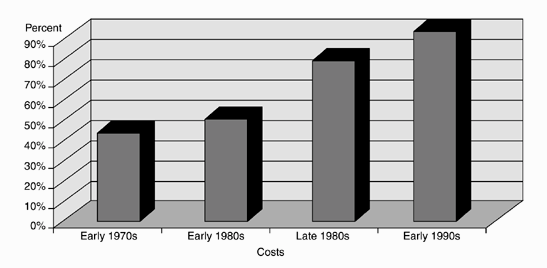
\includegraphics[width=0.7\textwidth]{Chapters/2-Lehmanns-Gesetze/images/costsDevotedToSoftwareModernization.png}
  \caption{Software-Kosten, welche der Software-Modernisierung gewidmet werden. \cite{seacord_modernizing_2003}}
  \label{fig:costsOfModernization}
\end{figure}

\pagebreak

\section{Langfristige Auswirkungen von Lehmanns Gesetzen}
Wird das System nicht an die gewandelte Umgebung angepasst, entsteht zunehmen eine Diskrepanz zwischen der Umgebung der Software und dem Softwaresystem selbst. Grafik \ref{fig:fehlendeVerbesserung} illustriert diesen Zusammenhang.\\
Fehlt den Mitarbeitern das Verständnis für die Architektur und bestehende Codebasis, wird es zunehmend schwieriger die Software anzupassen. Möglicherweise ist die Software nicht umfassend testbar. 
Änderungen können folglich unvorhergesehene Wechselwirkungen hervorrufen. \cite{daniel_kramer_legacy-software_2020} \\
Dies führt unter den Mitarbeitern zu dem sogenannten “Fear-Driven-Development“\cite{daniel_kramer_legacy-software_2020}. Anpassungen werden dadurch nur spärlich eingearbeitet und meist vermieden.\\  
Die Software wird demnach resistent gegen Änderungen am Code. Eine Erhaltung oder Steigerung der Effizienz setzt allerdings Änderungen voraus. 
Darüber hinaus sind Fehlerursachen ohne umfassende Kenntnisse der Codebasis schwieriger auszumachen. Die Zeit und Kosten Fehler zu beseitigen steigen.\\
Zusammenfassend lässt sich also sagen, dass die Software unwirtschaftlicher wird. Immer größere Investitionen werden nötig um immer weniger Steigerungen in der Nützlichkeit der Software zu erreichen. Folglich wird die Software von Konkurrenz-Produkten überholt und zunehmend weniger konkurrenzfähig.
\begin{figure}[bth] 
  \centering
  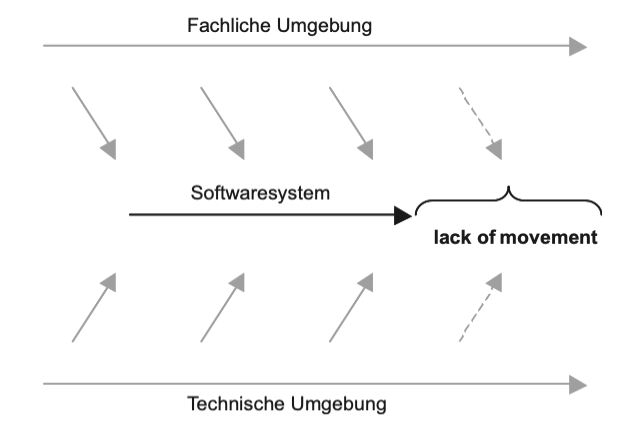
\includegraphics[width=0.7\textwidth]{Chapters/2-Lehmanns-Gesetze/images/fehlendeVerbesserung.png}
  \caption{Folgen einer fehlenden Anpassung der Software an ihre Umgebung \cite{bommer_softwarewartung_2016}}
  \label{fig:fehlendeVerbesserung}
\end{figure}

\section{Zusammenfassung}
Zusammenfassend lässt sich sagen, dass sich die Problemstellung der Software-Alterung auf zwei verschiedene Aspekte bezieht.\\
Zunächst wird durch Lehmanns Gesetze klar, dass eine Software angepasst werden muss. Sonst schreitet das Umfeld der Anwendung fort, während die Anwendung stehen bleibt. Die Software veraltet. Führt man allerdings Änderungen an der Software durch Ergeben sich neue Probleme. Denn werden die Grundprinzipien der Architektur missachtet, degeneriert die Architektur. Diese Degeneration führt erneut zu einer Alterung der Software. Folglich stellt sich die Frage, wie dieser Alterung entgegengewirkt werden kann, ohne die Architektur zu schädigen.






%Die Software-Entwicklung
\cleardoublepage\chapter{Die Software-Entwicklung}
\label{chapter3}
Das vorherige Kapitel führte Lehmanns Gesetze ein. Basierend auf deren Annahmen wurden innere und äußere Gründe herausgearbeitet, welche zu diesen Gesetzen führen. Abschließend wurden einige Auswirkungen dieser Gesetze aufgezeigt.\\
In diesem Kapitel wird dargestellt, was Software Modernisierung ist. Dafür wird zunächst der Softwareentwicklungsprozess nach Seacord et al. dargestellt. Anschließend wird die Software-Modernisierung in Seacord’s Entwicklungsprozess  eingeordnet.

\section{Der Software-Entwicklungsprozess}
Die Software-Modernisierung kann als Teil des Software-Entwicklungsprozesses betrachtet werden. 
Seacord et al. \cite{seacord_modernizing_2003} teilt diese in 3 voneinander getrennte Phasen auf.\\
Hierzu zählt zunächst die Instandhaltung der Software. Diese geht über in die Software-Modernisierung. Bis schließlich eine Ersetzung des Systems angestrebt wird. Grafik \ref{fig:lifecycle} illustriert diese 3 Phasen.\\
Die gepunktete Linie in Grafik 3.1 zeigt die Anforderungen der Firma, die sogenannten \textit{Business needs}. Die durchgezogene Linie hingegen gibt die Funktionalität des Systems an.\\
Eine wiederholte Instandhaltung der Software nährt die beiden Linien kurzfristig an. Die Funktionalität ist in diesen Zeitspannen ausreichend um die Business Needs zu befriedigen. 
Mit der Alterung des Systems können zunehmend solche kurzfristigen Lösungen nicht mehr die Funktionalität ausreichend steigern. \\
Eine Modernisierung der Software nimmt mehr Zeit und Geld in Anspruch, als eine Wartung. Mit umfangreichen Änderungen des Systems kann allerdings erneut die Funktionalität an die Anforderungen angeglichen werden. 
Wenn das alte System schließlich nicht mehr weiterentwickelt werden kann, muss es ersetzt werden. 
Die Entscheidung, welche der drei Optionen für ein bestimmtes System angewandt wird, kann nur durch eine eingehende Analyse bestimmt werden. Zeit, Kosten und Abhängigkeiten zur Software sind nur ein kleiner Teil der relevanten Parameter. Oft sind Systemausfälle im Zusammenhang mit längeren Modernisierungsmaßnahmen schlicht nicht akzeptabel. \cite{seacord_modernizing_2003} \\
Im Folgenden werden die Unterschiede von Wartung, Modernisierung und Ersetzung aufgezeigt. 

\begin{figure}[bth] 
  \centering
  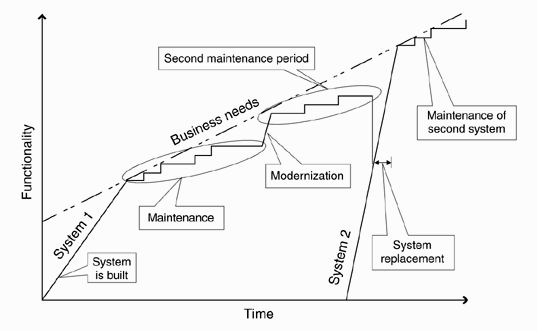
\includegraphics[width=0.7\textwidth]{Chapters/3-Die-Software-Entwicklung/images/LebenszyklusEinesInformationssystems.png}
  \caption{Lebenszyklus eines Informationssystems \cite{seacord_modernizing_2003}}
  \label{fig:lifecycle}
\end{figure}

\section{Software-Wartung}
Die Wartung arbeitet kleine Verbesserungen, wie Fehlerbehebungen oder strukturelle Verbesserungen ein. Diese Anpassungen verändern nichts an der grundsätzlichen Struktur der Software. Folglich bleibt die eigentliche Architektur unangetastet. \cite{seacord_modernizing_2003}\cite{bommer_softwarewartung_2016}\\
\newline
Der Prozess der Wartung ist iterativ. Sie unterstützt die Entwicklung des Systems, hat aber auch Einschränkungen, denn sie erschließt keine Wettbewerbsvorteile. \cite{seacord_modernizing_2003}
Der Umzug in die Cloud oder die Umstellung des Softwareangebots auf Software as a Service sind keine Wartungs-Operationen. Letztere erfordern tiefgreifende strukturelle Anpassungen und können die Architektur des Software-Systems beeinflussen.\\
Allerdings lässt sich die Software-Wartung in Kategorien aufteilen. Diese sind in der Norm IEEE610 festgehalten.:
\begin{description}
    \item [korrektive Wartung] \hfill \\ Boomer et Al. beschreibt diese, als das Beheben von Softwarefehlern. Letztere sind Restfehler, welche nicht während der Entwicklung bemerkt wurden. Die Art des Fehlers kann weiter als Mängel oder Instandhaltung verstanden werden. Ersteres sind kleine Fehler, welche gesammelt und zu gegebener Zeit behoben werden können. Instandhaltung meint allerdings schwere Mängel, welche den Betrieb stören können. \cite{bommer_softwarewartung_2016}
    \item [adaptiver Wartung] \hfill \\ Bei der adaptiven Wartung werden kleine fachliche oder technischen  Anpassungen unternommen. Für erstere wäre die Änderung des Mehrwertsteuersatzes zu nennen. Es kann auf eine neue System-Version umgestellt werden. Diese System-Umstellung ist lediglich dazu da, denn vorherigen Zustand des Systems wiederherzustellen. Hierbei entsteht kein Mehrwert. \cite{bommer_softwarewartung_2016}
    \item [perfektionierender Wartung] \hfill \\ Das Ziel der perfektionierenden Wartung ist die Verbesserung nicht-funktionaler Anforderungen. Mit kleinen Änderungen wird dabei z.B. die Antwortzeit der Software verbessert. \cite{bommer_softwarewartung_2016}
    \item [präventive Wartung] \hfill \\ Bei der präventiven Wartung werden proaktiv Fehler gesucht, welche noch nicht im laufenden Betrieb aufgefallen sind. Diese Tätigkeit ist folglich planbar. \cite{bommer_softwarewartung_2016}
\end{description}
Bommer et Al. \cite{bommer_softwarewartung_2016} kategorisiert diese zudem nach einer reaktiven oder proaktiven Beteiligung. Dies wird in Grafik \ref{fig:proactive} gezeigt. 
\begin{figure}[bth] 
  \centering
  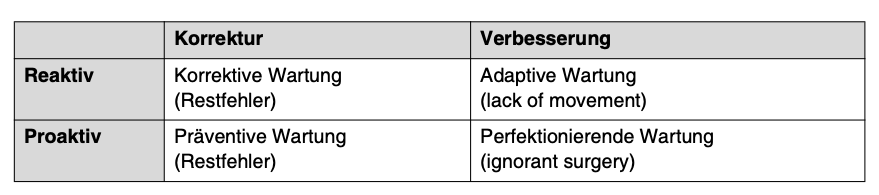
\includegraphics[width=0.7\textwidth]{Chapters/3-Die-Software-Entwicklung/images/KindsOfCorrection.png}
  \caption{Art der Software-Wartung nach proaktiv und reaktiver Beteiligung \cite{bommer_softwarewartung_2016}}
  \label{fig:proactive}
\end{figure}
Darüber hinaus steigt der Schwierigkeitsgrad einer Wartung zunehmend. Denn das Ziel dabei ist es die Software Funktionalitäten erneut an die Business Needs anzupassen. Strukturelle Verbesserungen und Fehlerbehebungen genügen dafür, bei einer stark gewachsenen Software, nicht mehr.

\section{Software-Modernisierung}
Die Software-Modernisierung ist der Prozess der Weiterentwicklung einer Software. Dies geschieht, indem Teile ersetzt, neu-entwickelt oder auf eine neue Plattform migriert werden. \cite{khadka_does_2015}
Khadka et Al. \cite{ravi_khadka_how_nodate} nennt die zu modernisierenden Systeme \glqq[...] Legacy Systems [...]\grqq{}, sofern diese schwer anzupassen sind und dennoch kritisch sind für das laufende Geschäft. Die Software-Modernisierung passt Legacy-Systeme an gewachsene System-Anforderungen an, wenn dies nicht mehr durch Wartungsmaßnahmen getan werden kann. Daraus ergibt sich, dass die Software-Modernisierung dann eingesetzt wird, wenn eine Wartung zu schwierig und kostspielig ist. \\
Die Software-Modernisierung arbeitet dabei größere Änderungen in das System ein. Zu beachten ist allerdings, dass ein Großteil des Systems beibehalten wird. Dies ist dann von Nutzen, wenn ein Software-System Anpassungen benötigt. Allerdings der Kern des Systems weiterhin ein Business Value hat. \cite{seacord_modernizing_2003}\\
Seastorm et Al. \cite{seacord_modernizing_2003} unterscheidet zudem \textit{White-Box Modernisierung} und \textit{Blackbox Modernisierung}. Die White-Box Modernisierung benötigt wissen über die internen Komponenten.  Wohingegen Black-Box Modernisierung nur Kenntnisse über externe Schnittpunkte benötigt. 

\section{Software-Neuentwicklung}
Die Neuentwicklung benötigt den Aufbau eines komplett neuen Software-Systems. Folglich ist dieser Ansatz kosten- und zeit-intensiv. 
Die Software-Neuentwicklung bietet sich an, wenn sowohl White-Box, als auch Black-Box Modernisierung nicht kostengünstiger als die Neuentwicklung sind.\\
Hier ist anzumerken, dass nicht alle Bestandteile des Systems gleichzeitig erneuert werden müssen. Eine Architektur bestehend aus klar abgetrennten Systemen kann auch teilweise neu entwickelt werden. \\
In diesem Stadium gilt zu evaluieren, ob eine kommerzielle Software für die gegebenen Anforderungen geeignet ist. Diese sogenannte \ac{COTS} Software \cite{abts_cocots_2000} sind in unter anderem als Customer-Resource-Management-Systeme oder Finanz-Systeme verfügbar. 
\acs{COTS} Software-Systeme sind bereits fertig implementierte Software-Bausteine für die genannten Anwendungsfälle. Eine firmeneigene Entwicklung kann so vermieden werden. \cite{abts_cocots_2000}\cite{seacord_modernizing_2003}







%Refactoring
\cleardoublepage\chapter{Refactoring}
\label{refactoring}
\label{chapter4}
In diesem Kapitel wird das Refactoring näher beleuchtet. Refactoring stellt eine Möglichkeit dar, die Alterung einer Software zu verlangsamen. Zunächst wird dabei der Begriff Refactoring erläutert. Mit dem gesammelten Wissen können anschließend einige konkrete Refactoring Maßnahmen beleuchtet werden. Dabei wird sich auf das Buch Refactoring \cite{fowler_refactoring_2018} von Martin Fowler und Kent Beck bezogen. Anschließend wird das Refactoring mit der Software-Modernisierung in Verbindung gesetzt. Das Kapitel schließt mit der Frage, wann Refactoring-Maßnahmen angewendet werden sollten.

\section{Was ist Refactoring}
Mit dem Begriff Refactoring kann sowohl das Substantiv, wie auch das Verb betrachtet werden. Grundsätzlich findet bei dem Refactoring eine Änderung an der internen Struktur von Software statt. Beispielsweise kann das innere Verhalten effizienter sein. Auch besser lesbarer Code oder die Bündelung von zuvor verstreuten Verhalten sind Beispiele für Refactorings. Laut Flower und Beck ist das Ziel des Refactorings stets den Code einfacher verständlich und billiger modifizierbar zu machen. Diese Änderungen sind von außen nicht wahrnehmbar. Das äußere Verhalten bleibt unverändert.  \\
Das Ziel dieser Änderungen ist, dass er Code leichter lesbar und zu modifizierbar wird. Da sowohl lesen, als auch modifizieren weniger Zeit in Anspruch nehmen, werden diese billiger.\\
Allerdings führen die internen Änderungen des Refactorings zu keiner Veränderung des äußeren Verhaltens der Software. 
Das Verb Refactoring meint nun die Anwendung einer Reihe von konkreten Refactorings. Der Autor und Informatiker Martin Fowler und der Informatiker Kent Beck haben in ihrem Buch Refactoring eine Reihe dieser konkreten Refactorings definiert. \cite{fowler_refactoring_2018}\\
\newline
Refactoring sollte dabei nicht als Synonym für jede Art von Code-Restrukturierung und Bereinigung verwendet werden. Flower und Beck sehen in Refactoring eine sukzessive Anwendung von einzelnen Refactorings.\cite{fowler_refactoring_2018} Jeder dieser Schritte erhält das Verhalten der Anwendung. Der Code bleibt daher nach jedem einzelnen Refactoring ausführbar mit dem identischen Verhalten wie zuvor. Refactoring ist eine besondere Art der Restrukturierung.\\

\section{Bad-Smells}
Um Kandidaten für Refactoring-Maßnahmen zu finden, muss der Begriff Bad-Smell betrachtet werden. Der Autor und Entwickler Martin Flower definiert ein Bad-Smell als einen oberflächlichen Hinweis, der in der Regel mit einem tieferen Problem im System korrespondiert. \cite{martin_fowler_codesmell_nodate}\\
Martin Flower und der Entwickler Kent Beck begründen die Wahl Wortes \textit{Smell} damit, dass dieser schnell zu erfassen ist. Ein Mensch kann einen Geruch wahrnehmen, ohne darüber nachzudenken. Ferner muss nicht klar sein, wo die Ursache des Geruches ist. Man weiß nur, dass man etwas riecht.\\
Martin Flower nennt hier als Beispiel Methoden mit überdurchschnittlich vielen Parametern. Letzteres fällt einem aufmerksamen Entwickler ins Auge, ohne das er aktiv darüber nachdenkt. Ein weiterer Grund für die Wahl des Wortes Smell war, dass ein Geruch nicht zwangsläufig etwas Schlechtes ist. Methoden mit überdurchschnittlich vielen Parametern können gerechtfertigt sein. Der Bad-Smell kann sich folglich auch als ungefährlich herausstellen. \\
Tools wie zum Beispiel \textit{SonarQube} \cite{sonarqube_code_nodate} helfen dem Entwickler dabei Bad-Smells zu finden. Anschließend können Refactoring-Maßnahmen angewendet werden.

\section{Refactorings und die Software-Modernisierung}
Die grundsätzliche Aufgabe von Refactorings ist es Lehmans Gesetzen entgegenzuwirken. Konkret soll der Verfall der Architektur verlangsamt werden. 
Wird eine Architektur zunehmend modifiziert, hat dies eine kumulative Wirkung. Umso härter es ist, das Design im Code zu sehen, umso härter ist es dieses zu erhalten. Folglich verfällt das eigentliche Design zunehmend schneller. Regelmäßiges Refactoring hilft dabei den Code sauber zu halten. Ferner soll dem Wachstum der Code-Basis entgegengewirkt werden. \cite{fowler_refactoring_2018}\cite{daniel_kramer_legacy-software_2020}\\
\newline
Fowler stellt in seinem Buch Refactoring \cite{fowler_refactoring_2018} einige konkrete Refactoring Maßnahmen vor, mit welchem Code Vervielfältigung entgegengewirkt wird. Primär ist das Ziel jede Deklaration von Verhalten genau ein Mal und auch nur ein Mal zu definieren. Mittels Refactoring werden etwaige doppelte Deklarationen gefunden und auf eine Deklaration reduziert. 
Oft fallen solche Zusammenhänge nicht während der Entwicklung auf. Das Refactoring hilft dabei, dies nachzuholen. \\
\newline
Darüber hinaus definiert Kent Beck die Design \textit{Stamina Hypothesis} \cite{fowler_refactoring_2018}. 
Diese Hypothese beschreibt, dass indem wir uns um ein gutes internes Design bemühen, wir länger schneller arbeiten können. 
Grafik \ref{fig:stamina} verdeutlicht diesen Zusammenhang. Die blaue Linie wächst zu Beginn schneller. Denn sie nutzt ein wenig durchdachtes Design. Dadurch können schnell Fortschritte erreicht werden, allerdings wird die Codebasis zunehmend schwieriger anzupassen. Die rote Kurve nutzt ein durchdachtes Design. Folglich wächst sie zu Beginn langsamer, anschließend allerdings stetig.
Zuvor ein perfektes Software-Design zu erstellen, ist unwahrscheinlich. Daher wird Refactoring essenziell, um dieses während der Entwicklung zu erreichen.\\
\newline
Abschließend hilft Refactoring bei der Fehlersuche. Während der Einarbeitung von Refactorings beschäftigt sich der Entwickler eingehend mit bereits geschriebenen Code. Dadurch wird das Verständnis für den zugehörigen Code erweitert. Dieses erweiterte Verständnis kann mittels weiteren Refactoring-Maßnahmen in den Code einfließen. Dadurch können Annahmen und Überlegungen des Entwicklers klarer im Code selbst repräsentiert werden. Die klare Repräsentation von Annahmen erleichtert anschließend die Fehlersuche.
Zusammenfassend lässt sich sagen, dass Refactoring-Maßnahmen dabei helfen Lehmanns Gesetzen entgegenzuwirken. Der bereits bestehende Code wird klarer formuliert und das Verständnis für den Code wird vertieft. Dadurch können Fehler schneller gefunden werden und dem Verfall der Architektur wird entgegengewirkt.

\pagebreak

\section{Software-Modernisierung im Vorgehensmodell}
Mit dem gesammelten Wissen stellt sich die Frage, wann konkret Refactoring-Maßnahmen angewendet werden sollten. \\
Martin Fowler beschreibt dies wie folgt: "Refactoring is something I do every hour I program.". Darüber hinaus nennt Fowler "The best time to refactor is just before I need to add a new feature to the code base.". \cite{fowler_refactoring_2018}\\
Der Entwickler Daniel Krämer beschreibt in dem Magazin Objektspektrum vom Mai 2020 ein konkretes Vorgehen für Refactorings innerhalb einer laufenden Entwicklung. 
Er sieht es ebenfalls als ratsam an, bereits während der Planung eine Vorstellung vom Umfang der beabsichtigten Aufräumarbeiten zu gewinnen und deren Kosten explizit in die Schätzung eines Tasks einfließen zu lassen.\\
Daraus ergibt sich, dass Refactoring und das Implementieren von neuen Funktionen, zwei voneinander getrennte Aufgabenbereiche sind. Während der Planung sollten beide Aufgabenbereiche eine Rolle spielen und beiden sollte genügend Zeit eingeplant werden. Darüber hinaus erleichtern das Schreiben von Regressionstest die Arbeit mit Refactorings.  \cite{daniel_kramer_legacy-software_2020}\cite{fowler_refactoring_2018}


\begin{figure}[bth] 
  \centering
  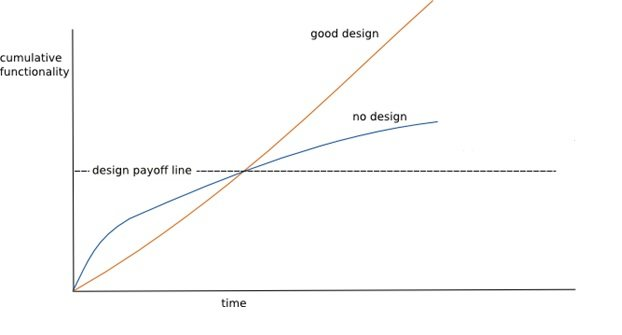
\includegraphics[width=0.7\textwidth]{Chapters/4-Refactoring/images/DesignStaminaHypothesis.jpg}
  \caption{Design Stamina Hypothesis \cite{fowler_refactoring_2018}}
  \label{fig:stamina}
\end{figure}




%Vorgehensmodell Cloud Native
\cleardoublepage%*****************************************
\chapter{Vorgehensmodell für Cloud Computing}\label{ch:vorgehensmodell}
%*****************************************
\section{Vorab}
\label{VgmVorab}
%=============================

Auf den in den vorigen Teilen beschriebenen Grundlagen, Techniken und Vorteilen von Software-Modernisierung aufbauend wird folgend mit Cloud Computing ein Praxisbeispiel behandelt.
Abhängig der jeweiligen Branche greifen heutzutage immer mehr Unternehmen auf Cloud Lösungen von Drittanbietern(Provider) zurück. Diese bieten den Unternehemen, neben der Angebotsvielfalt, einige qualitative und quantitative Benefits. Daher erfreut sich deren Verwendung heutzutage immer größer werdender popularität und Beliebtheit \cite{skyhigh}. Die Entscheidung der Betrachtung für Cloud Computing in dieser Ausarbeitung erfolgte nach keinem  Ranking, das Cloud Computing im Vergleich von anderen Technologien hervorhebt. Der Einsatz dieser Lösung in der Praxis richtet sich nach den Bedürfnissen und Zielen der Unternehmen. Für die weiteren Betrachtungen wird von Unternehmen in der freien Marktwirtschaft ausgegangen. 
\\\\
Als exemplarische, moderne, zukunftsorientierte Technologie liefert Cloud Computing Grund genug eine facettenreiche  Betrachtung  einer Software-Modernisierungsmaßnahme durchzuführen. Die entstehenden zahlreichen Fragestellung, Analysen, Auswertungen und Evaluationen beeinflussen maßgeblich die zukünftige IT-Landschaft eines Unternehmens. 
\\\\
Eine Modernisierungsmaßnahme, bei der ein Legacy-System zu einer künftigen Cloud-Lösung entwickelt werden soll, erfordert gewisse Grundlagen. Neben der Definition des \textit{National Institut of Standards and Technologies} zu Cloud Computing, wird  notwendige Wissen in Abschnitt \ref{VgmCC} \nameref{VgmCC}  vermittelt.  Anschließend wird in Kapitel  \ref{VgmOnPremise} \nameref{VgmOnPremise} die Lösungsmöglichkeit von einer „on-premise in house-Lösung“ zu Cloud Computing abgegrenzt. Die konkrete Durchführung einer Software-Modernisierungsmaßnahme stellt für die  Unternehmen ein kompliziertes und komplexes Projekt dar. Zur Weiteren Vermittlung wird in Abschnitt \ref{VgmVorgehensmodell} \nameref{VgmVorgehensmodell} eine vereinfachte Roadmap, also ein Vorgehensmodell zur Umsetzung einer Modernisierungsmaßnahme einer Cloud Computing Lösung vorgestellt. Die Möglichkeiten wie Services, beziehungsweise Dienste, in der späteren Cloud angeboten werden können, wird in \ref{VgmAsAService} \nameref{VgmAsAService} voneinander abgrenzt. In \ref{VgmPublicProvider} \nameref{VgmPublicProvider}  schließt sich der Kreis, mit der abschließenden Vorstellungen von Amazons „Amazon web services (aws)“ und Microsofts „Azure“.
\newpage
\section{Cloud Computing im Überblick}
\label{VgmCC}
%=============================
Für einen gemeinsamen Kontext zu dem Begriff Cloud Computing wird die Definition des National Institut of Standards und Technology im Rahmen dieser Ausarbeitung verwendet. Dieses führt fünf grundlegende und einheitliche Charakterstika für Cloud Computing Systeme ein. Die zusammenfassenden Oberbegriffe dieser sind der On-demand self service, Broad network access, Resource pooling, die Rapid elasticity und dem Measured service.
\\\\
Im Wesentlichen fassen die genannten Punkte die Möglichkeiten zusammen für einen entfernten, einseitigen Zugriff aus dem Netz mit heterogenen Endgeräten auf Rechen- und Serverressourcen. Diese Ressourcen werden, in Abhängigkeit der Bedürfnisse und Notwendigkeit, skalierbar und bedarfsgerecht, nach dem Mehrmandantenprinzip bereitgestellt. Die Benutzer und Benutzerinnen sehen dabei nicht, mit welchen (physischen) Kapazitäten die Leistung erbracht wird. Der measured Service beschreibt die Anforderung für die Bereitstellung erhobener Daten. Diese schließen unter anderem Kennzahlen wie die Zugriffszeiten, Anzahl aktiver Nutzer und Nutzerinnen, Server- und Speicherauslastung erhöhen die Transparenz mit ein. Dies ist nicht nur für die Transparenz seitens der Unternehmen wichtig, die für diese Dienste bezahlen, sondern auch für die Drittanbieter dieser Lösungen, die somit ihre Ressourcen überwachen und gegebenenfalls mit physischer Hardware der erwartbaren Nachfrage aufrüsten müssen. \cite{nist}
\\\\

Cloud Computing basiert auf der \ac{SOA} \cite{CcIBM}, also der Service-, beziehungsweise Dienst-Orientierten Architektur. Ein Dienst/Service ist eine in sich geschlossene Softwareeinheit, die mit Anwendungen und/oder anderen Diensten über einen lose gekoppelten, oft asynchronen Kommunikationskanal kommuniziert. \acs{SOA} bezeichnet dabei die gesamte Architektur, bestehend aus den miteinander kommunizierenden Diensten. Grundlegende Eigenschaften der \acs{SOA} ist ein einheitlicher Kommunikationskanal und die lose gekoppelten Dienste. Bei deren Entwicklung liegt der Fokus auf einem qualitativ hochwertigen, bereitgestellten Dienst. \cite{lewis2005service} \\\\

Dies ist nicht ohnehin von besonderer Bedeutung, da man Fehler aus der Vergangenheit (Beispielweise. schlechte Code-Entwicklung, schlechtere Services, etc.) nicht im neuen System wiederholen möchte.  \acs{SOA} bietet somit in seinen Grundzügen einen soliden Kern, auf dem Cloud Computing aufbaut. 
\\\\
Neben der Bestimmung der quantitativen und qualitativen Vor- und Nachteile, spielen oft weitere Faktoren eine wichtige Rolle.  Auch die Auswahl von der Unternehmensgröße (aus Kostengründen) und der Branche des Unternehmens spielt eine wichtige Rolle. Beispielsweise unterliegen Behörden oder Betrieben der Sektoren Banken, Versicherungen oder sonstigen Finanzdienstleister besonderen (Datensicherheits-)Gesetzen. Für die Einhaltung von (IT-)Compliance oder etwaigen internen Kontrollsystemen, kommt eine on-premise und in-house Lösung für die Modernisierungsmaßnahme, beziehungsweise der zukünftigen IT-Landschaft infrage. \cite{falk2012compliance}\newpage

\section{On-premise in-hose vs Cloud Computing bei Providern}
\label{VgmOnPremise}
%=============================


Um auch Cloud Computing, von einer im Unternehmen entwickelten und betriebenen Software zu unterscheiden (On-premise in-house), werden im Folgenden die Punkte Deployment, Kontrolle, (Daten-)Sicherheit und (IT-)Compliance Anforderungen voneinander abgegrenzt. Es soll deutlich gemacht werden, welche Vor- und Nachteile die Unternehmen im Zuge der Überlegungen für die Software-Modernisierung betrachten sollen und welche Restriktionen  beeinflussen. On-Premise Software ist auf den Unternehmenservern installiert. Der Zugriff ist, neben der Firewall, von verschiedene in-house Faktoren abhängig. Diese Applikationen gelten als zuverlässig und sicher und ermöglichen den Unternehmen, ein hohes Maß an Kontrolle. \cite{fisher2018cloud}
\\\\
Folgend werden die beiden Lösungsvarianten unter verschiedenen Gesichtspunkten voneinander abgegrenzt.
\begin{description}   
 \item [Deplyoment] \hfill \\
In einer on-premise Enviroment findet das Deployment innerhalb der Unternehmen-IT-Infrastruktur statt. Entsprechend sind die Verantwortlich für die Wartung der Lösung und alle mit ihr verbundenen Prozesse. \\Die virtuelle Cloud-Infrastruktur hingegen bietet hohe Flexibilität bei der Implementation auf einer  breiten Infrastruktur. Zusätzlich ermöglicht es eine schnellere Installation und Support-Services, was auch die Systemadministrator effizient unterstützen kann.\cite{bibi2012business}
 \item [Kontrolle] \hfill \\
Die Unternehmen mit einer on-premise Lösungen erheben, verfügen, analysieren und evaluieren die Unternehmen alle Daten. Was besonders für die Verwendung einer on-premise Lösung für Unternehmen spricht, die in einer stark-regulierten Branche arbeiten.\\
In der Cloud-Computing-Umgebung stellen sich viele Unternehmen und Provider die Frage nach des Eigentums der Daten. Diese befinden sich physisch bei den Drittanbietern. Falls es zu Problemen und Ausfällen kommt, können Unternehmen möglicherweise nicht auf diese Daten zugreifen.\cite{bibi2012business}
 \item [(Daten-)Sicherheit] \hfill \\
Unternehmen mit besonders sensiblen Informationen, wie Behörden und Banken, müssen über ein gewisses Maß an Sicherheit und Datenschutz verfügen, das eine on-premise in-house Lösung bietet.
Sicherheitsbedenken sind im Allgemeinen auch bei durch Drittanbieter angebotenen Cloud Computing-Lösungen ein Problem. Auch, wenn die Provider im Laufe der Zeit die Robustheit der gesamten Infrastruktur unter Beweis gestellt haben. \cite{klotz2008compliance} \cite{falk2012compliance}
 \item [Compliance] \hfill \\
Viele Unternehmen arbeiten, unabhängig von der Branche, unter behördlichen Kontrollen. Für Unternehmen, die solchen Vorschriften unterliegen, ist es zwingend erforderlich, dass sie ihre (IT-)Compliance permanent im Auge haben. Hierfür eignet sich die on-premise Variante eher. \\
Auch dann sind  Unternehmen für die Einhaltung von (IT-)Compliance Richtlinien verantwortlich, wenn sie eine Cloud-Lösung bei einem Drittanbieter haben. Sensible Daten müssen geschützt werden um Kunden/Kundinnen, Partner/Partnerinnen und Mitarbeiter/Mitarbeiterinnen  ihre Privatsphäre gewährleisten zu können.\cite{klotz2008compliance}
\end{description}

\section{Vorgehensmodell zur Umsetzung für Cloud Computing}
\label{VgmVorgehensmodell}
%=============================
\begin{flushright}{\slshape    
    [With legacy systems] the cost is getting higher because maintenance is getting more expensive, [then] maybe you should think of modernization}
    --- unbekannt \cite{profperLeg}
\end{flushright}

Die Entwicklung, der Betrieb, die Betreuung und die stetige Weiterentwicklung durch neue Anforderungen von  Software im Unternehmen erfordert  mehr Expert:innenwissen als früher. Ursache dafür ist auch der immer größer werdende Anteil künstlicher Intelligenz in Applikationen. Es wird Hardware benötigt. Ebenso weitere physischer Computerressourcen für Fallback-Szenarien, die auf die Gewährleistung von (IT-)Compliance einzahlen.
\\\\
Repräsentative und auswertbare Studien bereits umgesetzter Modernisierungen größerer Unternehmen finden sich in der Literatur nur wenige. Etwaige Gründe dafür könnten sein, dass diverse erfolgreiche Lösungen aufgrund des Konkurrenzdenkens und resultierenden Marktvorteil nicht veröffentlicht werden.  Obwohl immer mehr Unternehmen die Bedeutung und die Vorteile von signifikant besser wartbarer und skalierbarer Software erkennen, führen sie keine Modernisierungsmaßnahmen durch. Eine mögliche Erklärung dafür kann an dem mangelnden Fachpersonal liegen.  \\\\

Trotz einer gut definierten Enterprise-Architektur und unmissverständlich dokumentierten Sourcecode ( \nameref{refactoring}) einer Legacy-Software, begegnen dem (IT-)Personal viele Hürden. Der Weg der Legacy Software bis hin zur „modernen Software“ muss klar definiert, strukturiert und deterministisch sein. \\\\
Die Software-Modernisierung einer Legacy ist keineswegs trivial. Zahlreiche Herausforderungen, die nicht nur Geld kosten, erschweren den Weg von der Legacy zur modernen Software. Wie kann die zukünftige Software qualitativ verbessert werden?  Was  gilt überhaupt zu beachten? Welche Anforderungen galten bisher? Wie soll die Ziellandschaft aussehen? Eine ausgeklügelte Strategie kann für den langfristigen  Erfolg und Erhalt der Software sorgen.  Die Unternehmen benötigen eine Roadmap/ ein Vorgehensmodell. Es soll alle notwendige Schritte definieren, alle Fragestellungen kategorisch zusammenfassen und die Unternehmen in jedem Schritt der Modernisierungsmaßnahme unterstützen. 
\\\\
In der Literatur gibt es diverse Vorgehensmodelle zur Umsetzung von Modernisierungsmaßnahmen. Die Vielfalt dieser liegt unter anderem in den unterschiedlichen Anforderungen, verfügbaren Ressourcen, dem Risiko-Management, der zu modernisierenden Software und auch mit der mittel- bis langfristigen Unternehmensstrategie. \cite{10.1145/2818567.2818579}

\subsection{ARTIST EU} 
Ein Modell-getriebener Ansatz Europäischen Union nennt sich\textit{ \ac{ARTIST}}.\cite{artistEU} Die \acs{ARTIST} Methoden und  \acs{ARTIST} Frameworks, sollen die Entwickler und Entwicklerinnen in jedem Schritt der Migration- und Modernisierungsmaßnahme unterstützen. Dabei fasst es bereits Best-practises zusammen\cite{menychtas2014software}. In Teilen verwendet \acs{ARTIST} die \ac{SMART} die in der Pre-Migration-Phase stattfindet. \\\\
 \acs{SMART} wird unter anderem auch für die Analyse der Legacy verwendet, um festzustellen, ob beispielsweise ihre Funktionalität oder Teile davon als Services (\acs{SOA}) bereitgestellt werden können. Die Interaktion eines Legacy-Systems innerhalb einer \acs{SOA}, wie beispielsweise einer Web-Services-Architektur, ist manchmal relativ einfach – was wiederum sehr attraktiv für die Unternehmen ist. Web-Service-Schnittstellen sind so eingerichtet, dass sie SOAP-Nachrichten empfangen und analysiert werden, wodurch der entsprechende Dienst direkt aufgerufen werden kann. Zahlreiche neue Entwicklungsumgebungen bieten Tools, die diesen Prozess unterstützen. Unternehmen setzen eben diese Umgebungen  ein, um ihre Geschäftsprozesse der Welt zugänglich zu machen.\cite{lewis2005service} 
 
 
 
 
 
\subsection{Roadmap}
Das Vorgehensmodell zur Modernisierung einer Legacy von S. Jain und I. Chana \cite{ccRoadmap} wird  nun betrachtet. Einen groben Überblick bietet folgende Abbildung, die die wesentlichen Hauptkomponenten des Vorgehensmodells darstellt.


\begin{figure}[h] 
  \centering
  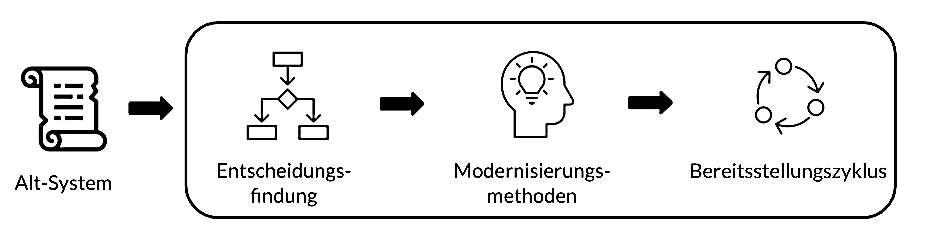
\includegraphics[width=0.7\textwidth]{Chapters/Vorgehensmodell/images/ccvorgehensmodell.png}
  \caption{Vorgehensmodell zur Umsetzung einer Modernisierungsmaßnahme für Cloud Computing. \cite{ccRoadmap}}
  \label{fig:picCCRoadmap}
\end{figure}

Erstens, das Entscheidungsmodul. Wieder rum besteht aus drei Hauptkomponenten, die im Wesentlich zur Bewertung des Alt- und Zielsystem eine Grundlage bilden.\\
Zweitens, das Modul für Modernisierungsmethoden. Hier stehen uns vier Schlüsselmethoden zur Auswahl, um die Modernisierungsmaßnahme mit einem geeigneten Ansatz und einer geeigneten Implementierung fortzusetzen.
Drittens, der Bereitstellungszyklus. Er beschreibt nach den ersten beiden Modulen einen permanenten Zyklus, bestehend aus vier zusammenfassenden Schritten.
\\\\
\addsec{Entscheidungsfindung}
Das erste Modul kann im Weiteren in drei weitere Module unterteilt werden.
\begin{description}   
 \item [Beurteilung des Altsystems] \hfill \\
Die Bestimmung der Komplexität für die Modernisierungsmaßnahme ist ein Hauptfaktor  um den Aufwand und die Kosten für das Projekt bestimmen zu können.  Dabei müssen die unterschiedlichen Schichten der Software, oder der IT-Infrastruktur betrachtet werden. Verglichen mit dem OSI-7-Layer Modell müssen die sieben Schichten Physical-, Data Link-, Network-, Transport-, Session-, Presentation-, Session- und Application-Layer untersucht werden \cite{briscoe2000understanding}.  Hier sollte bestimmt werden, in welchen Schichten beispielsweise die Business Logik liegt und mit welchen anderen Layern sie korrespondiert. Die Komponenten, die in das Cloud-System migriert werden sollen, beeinflussen somit die Skalierbarkeit der Applikationen in. 
 \item [Beurteilung (bisherige) Servicequalität] \hfill \\
Ebenfalls muss die bisherige Qualität analysiert werden. Was war bisher schlecht und was könnte  im Zuge der Modernisierung besser gemacht. Aus technischer sowie auch fachlicher Sicht. Konkret bedeutet das, ob man beispielsweise durch ein Redesign des Prozesses größere qualitative als auch quantitative Erfolge erzielen kann. Das könnten beispielsweise verkürzte Arbeitswege sein.
 \item [Bestimmung von Zielen] \hfill \\
 Aus den bisherigen Betrachtungen sollten nun die Ziele bestimmt werden. Das könnte auf allgemeinen Ebene z.B. sein: Ein besseres Management der Plattform, der Infrastruktur oder der Services. In Hinblick auf den Code können eine bessere Wartbarkeit, eine bessere Codequalität und quantitativ verringerte Komplexität von Funktion ebenso weitere Ziele sein. 
 \end{description}
 
\addsec{Medornisierungsmethoden}
S. Jain et al. stellen in ihrem Vorgehensmodell folgende vier Schlüsselmethoden vor
\begin{description}   
 \item [Ersetzung] \hfill \\
 Denkbar ist eine komplette Ersetzung von Software-Komponenten durch bereits existierende Software von Drittanbietern. COTS \cite{cots} gehen mit einem geringeren Risiko einher, da die Software bereits etabliert und getestet ist. Oftmals ist aber kein direkter Kauf mehr möglich, da viele Drittanbieter ihre Lösungen über diverse Lizenzmodelle anbieten. Das führt zu dem Nachteil, dass ein Unternehmen mittel- bis langfristig in hohem Maße von dem Anbieter abhängig sind. \\Ebenfalls kommt dieser Ansatz nicht infrage, sofern die bewertete Business-Logik sehr an die Bedürfnisse der Unternehmen angepasst wurde und damit nicht hundertprozentig mehr mit COTS ersetzbar ist.
 
 \item [Black Box Wrapping] \hfill \\
 In diesem Ansatz wird ein neues Interface lediglich an alte Komponenten der Legacy in der Cloud-Umgebung angebunden. Umsetzbar ist dieser Ansatz nur dann, wenn der Code der Legacy in einem gut-verwertbaren Zustand ist (vgl. \nameref{refactoring}). Ebenfalls beinhaltet dieser Ansatz eine sukzessive Anpassung der noch bestehenden Altsoftware im neuen System.
 \item [Reengineering/Redevelopment] \hfill \\
 Übergreifend mit dem Begriff Software-Engineering wird hier verwendet. Dieser Ansatz stellt somit eine komplette Neuentwicklung des Systems dar, mit teilweise Wiederverwendung oder Verbesserungen des alten Codes.
 \item [Migration] \hfill \\
\textit{} Das komplette System mit Kernfunktionalität wird in eine neue Umgebung repliziert, mittels unterschiedlicher Migrationsstrategien. So können auch Altsysteme bestehend und ohne Veränderung auf einer virtuellen Umgebung kurz- bis mittelfristig geparkt werden. Anschließend kann eine sukzessive Anpassung der Software erfolgen. An dieser Stelle erwähnenswert sind die Arten, wie spätere Dienste oder Applikationen in der Cloud angeboten und dargestellt werden können. Konkret handelt es sich hierbei um \ac{IaaS}, \ac{PaaS} und \ac{SaaS}. Diese Begriffe werden in Kapitel \textit{\ref{VgmAsAService} \nameref{VgmAsAService}} näher behandelt.
\end{description}   


\addsec{Bereitstellungszyklus}

\begin{figure}[h] 
  \centering
  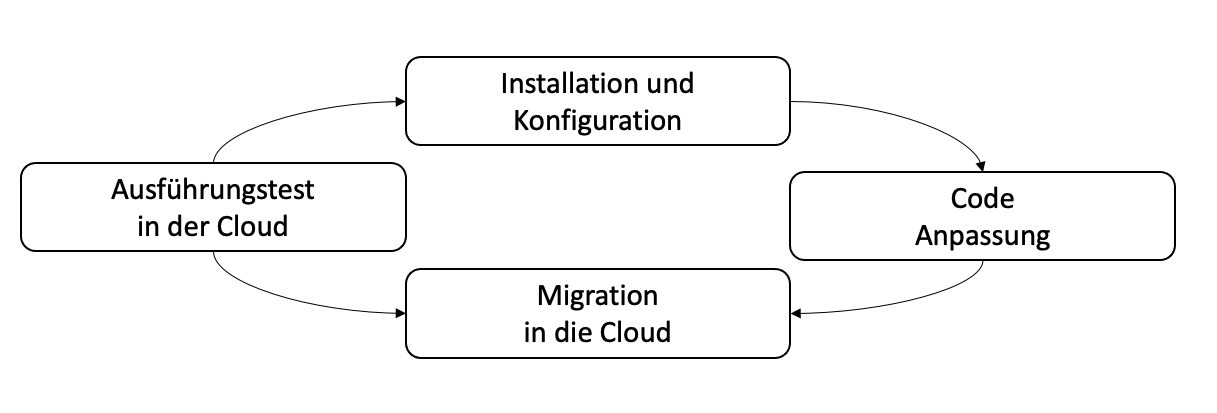
\includegraphics[width=0.8\textwidth]{Chapters/Vorgehensmodell/images/Bereitstellungszyklus.png}
  \caption{Bereitstellungszyklus im Vorgehensmodell \cite{ccRoadmap}}
  \label{fig:Bereitstellungszyklus}
\end{figure}
Nach der Selektion des geeigneten Ansatzes wird inkrementell mit der Implementierung begonnen, um die Modifikationen schrittweise mit den betroffenen Bestandteilen abzubilden. Mit der ersten Phase beginnend, kommt die Einrichtung und Einstellung der nötigen Tools für die Migration.  Einzelne Code-Segmente werden in den zirkulierenden Phasen priorisiert angepasst.
Es muss stets ein Fallback-Szenario vorhanden sein, bevor Änderungen am Quellcode durchgeführt werden. Hier kann ein Replikat der funktionierenden Alt-Version verwendet. 
Die modifizierte Komponente wird dann in der Cloud mit ausgewählten Servicemodellen (vgl. \textit{\ref{VgmAsAService} \nameref{VgmAsAService}}) und den jeweiligen Bereitstellungskonfigurationen gehostet. Abschließend findet in jedem Zyklus ein vollumfänglicher Test der Funktionalität innerhalb der Cloud statt, damit das System auch stets funktionsfähig bleibt und korrekt arbeitet.
 


\section{Schichtenmodell des Cloud Computings}
\label{VgmAsAService}
%=============================

Die Art und Weise, wie eine Software über ein Cloud-System bereitgestellt wird, ist Teil der Überlegungen für die Bestimmung der Ziele und Ziellandschaft. Cloud Computing unterteile dabei in drei Schichten, die Folgendermaßen erläutert werden. Es werden die Definitionen der einzelnen Schichten von IBM verwendet \cite{ibmAsAStructre}.

\begin{description}   
 \item [\acl{IaaS}] \hfill \\
 Hier bieten die Service-Provider Cloud-Lösungen, wie etwa Speicher, Netzbetrieb oder Server bereit. Dies bietet den Unternehmen den Vorteil Kosten für den Kauf und die Wartung eigener Hardware zu sparen. Und da die Daten alle in der Cloud liegen, gibt es keinen Single point of failure. Der Single point of failure ist im Prinzip eine Fehlfunktion, die zum Ausfall des Systems führen kann. 
 \item [\acl{PaaS}]\hfill \\
 Hier wird den Usern eine komplette Cloud-Umgebung bereitgestellt. Zusätzlich zu dem Speicher und IT-Ressourcen bekommen die Nutzer eine Reihe vordefinierter Tools an die Hand. Die ist insbesondere interessant für Tests und Entwicklungen.
 \item [\acl{SaaS}] \hfill \\
Hier wird eine Anwendungen Cloud-basiert angeboten. Der Zugriff erfolgt meist über die Programmschnittstellen oder Webinterfaces. Damit kann an über, beispielsweise den Webbrowser auf Applikationen des eigenen Unternehmens entfernt zugreifen, ohne sich in einem Virtuellen privaten Netzwerk zu befinden.
 \end{description}
\section{Bekannte Cloud-Computing Anbieter}
\label{VgmPublicProvider}
%=============================
Die Entscheidung bei welchem Anbieter Unternehmen ihre Cloud-Lösungen beziehen wollen, spielt  eine wichtige Rolle im Modernisierungsprozess. Technik-Giganten wie Amazon mit \textit{Amazon Web Services (AWS)}, Microsoft mit \textit{Azure} und Google mit \textit{Google Cloud }bieten mittlerweile schon länger Cloud-Lösungen für Unternehmen, als auch Privatpersonen an. Sie bieten alle die in Kapitel \ref{VgmAsAService} \nameref{VgmAsAService} vorgestellten Arten \acs{IaaS}, \acs{PaaS}, \acs{SaaS}. 
Interessante Gegenüberstellungen wie Bedienbarkeit, Geschwindigkeit und Zuverlässigkeit lassen sich in der Literatur, als auch von den Anbietern keine finden. Die für Kunden merkbaren Unterschiede stellen daher nur die Anbieterspezifischen Zusatzvorteilen, wie zum Beispiel Tools, Funktionen und Werkzeuge dar. 





\section{Zusammenfassung}
\label{Zusammenfassung}
%=============================
 Den Unternehmen, die Lösungen bei Cloud-Anbietern beziehen wollen, stehen heute eine Fülle an verschiedenen Möglichkeiten und Angeboten zur Auswahl. Neben der Angebotsvielfalt verschiedenerer Anbieter für Cloud-Systeme gibt es bereits auch viele Tools und Werkzeuge, die die Software-Modernisierung kostengünstiger und effizienter gestalten können. Unterstützt mit diversen Vorgehensmodellen, gestaltet sich so die Modernisierungsmaßnahme als keinen mehr zu groß unüberwindbar-wirkenden Monolithen mehr. Somit ist es so einfach wie noch nie veraltete Software günstiger modernisieren zu lassen.

%********************************************************************
% Bibliography/References
%*******************************************************
\cleardoublepage%********************************************************************
% Bibliography
%*******************************************************
\printbibliography

%********************************************************************
% List of Figures etc.
%*******************************************************
\cleardoublepage%*******************************************************
% Verzeichnisse (Abbildungen, Tabellen, Listings, etc.)
%*******************************************************
\cleardoublepage
\begingroup
	\let\clearpage\relax
	\let\cleardoublepage\relax
	\listoffigures
	%\listoftables
	%\addcontentsline{toc}{chapter}{\lstlistlistingname}
	%\lstlistoflistings 
\endgroup 
%*******************************************************
% Abkürzungsverzeichnis
%*******************************************************
\chapter*{Abkürzungsverzeichnis}
\addcontentsline{toc}{chapter}{Abkürzungsverzeichnis}	
	%Hier alle benötigten Abkürzungen einfügen
	\begin{acronym}[DSGVO] % LONGEST ACRONYM HERE FOR CORRECT SPACING
	    \acro{DSGVO}[DSGVO]{Europäische Datenschutzgrundverordnung}
	\end{acronym}
	\begin{acronym}[COTS] % LONGEST ACRONYM HERE FOR CORRECT SPACING
	    \acro{COTS}[COTS]{Commercial off-the-shelf}
	\end{acronym}
	

	\begin{acronym}[ARTIST] 
	    \acro{ARTIST}[ARTIST]{\textbf{A}lternative \textbf{R}outes \textbf{T}owards \textbf{I}nformation \textbf{S}torage and \textbf{T}ransport}
	     \acro{SMART}[SMART]{\textbf{S}ervice-\textbf{O}riented \textbf{M}igration and \textbf{R}euse \textbf{T}echnique}
	\end{acronym}

	\begin{acronym}[AsAService] 
	   \acro{IaaS}[IaaS]{Infrastructe as a Service}
	   \acro{PaaS}[PaaS]{Process as a Service}
	   \acro{SaaS}[SaaS]{Software as a Service}
	  \end{acronym}
	    
	    


% ********************************************************************
% Appendix/Anhang
%***************************************************************
%\appendix
%\part*{Anhang}
%\cleardoublepage%********************************************************************
% Appendix
%*******************************************************
\chapter{Erster Abschnitt des Anhangs}
In den Anhang gehören "`Hintergrundinformationen"', also weiterführende Information, ausführliche Listings, Graphen, Diagramme oder Tabellen, die den Haupttext mit detaillierten Informationen ergänzen. 

\blindtext
\blindtext
\blindtext



%*******************************************************
\cleardoublepage\pagestyle{empty}

\hfill

\vfill


\pdfbookmark[0]{Kolophon}{colophon}
\section*{Kolophon}
Dieses Dokument wurde mit der \LaTeX-Vorlage für Abschlussarbeiten an der htw saar im Bereich Informatik/Mechatronik-Sensortechnik erstellt (\currentVersion). Die Vorlage wurde von Yves Hary und Andr\'e Miede entwickelt (mit freundlicher Unterstützung von Thomas Kretschmer, Helmut G. Folz und Martina Lehser). Daten: (F)\makeatletter\f@size\makeatother\ -- (B)\the\textwidth\ -- (H)\the\textheight\ 


\end{document}
% ********************************************************************
